\chapter{Management Summary}

\section{Hintergrund}
Beim  Reiseveranstalter „hVs-Reisen“, der auf Reisen nach Nordkorea spezialisiert ist, kam es am Nachmittag des 14.11.2017 zu einem Security Incident, nachdem der
Virenscanner auf dem virtuellen Client des Mitarbeiters Lars Walter eine Malware
erkannt hatte.
Das Forensik-Team wurde daraufhin beauftragt, das betroffene System einer forensischen Analyse zu unterziehen. Der vorliegende Bericht gliedert sich in eine sog. Management Summary, in welcher die wichtigsten Ergebnisse der Untersuchung in kompakter Form dargestellt sind. Im Anschluss daran folgt eine detaillierte Aufstellung der Vorgehensweise und Ergebnisse, in der speziell auf die Fragen des Kunden eingegangen wird. Abgeschlossen wird der Bericht mit Handlungsempfehlungen für den Kunden von Seiten des Forensik Teams.

\section{Beschreibung des Security-Incidents}
Die Analyse des Security-Incidents bestätigte den Verdacht, dass der Rechner des Mitarbeiters Lars Walter durch eine Malware kompromittiert wurde.
Die Ursache der Infektion war eine Phishing-Mail, die der Mitarbeiter in seinem Google-Konto \path{hvsreisen.lwalter@gmail.com} erhalten hat.
Die E-Mail mit dem Betreff \textit{North Korea Update - Statement of Rex W. Tillerson} wurde am 13.11.17 um 16:19 Uhr empfangen.
Diese E-Mail enthielt einen Anhang mit der Zip-Datei
\path{Temp1_171110_NorthKorea-DiploimaticUpdate.zip}.
Diese Datei enthielt wiederum die Malware
\path{171110_NorthKorea-DiploimaticUpdate.pdf.exe}.
Diese wurde vom Benutzer am 13.11.17 um 16:27 Uhr ausgeführt, wodurch das System kompromittiert wurde.

Es ist davon auszugehen, dass es sich um einen zielgerichteten Angriff auf die hVs-Reisen handelt, da die Phishing-Mail stark indivualisiert ist und auf das Geschäftsfeld des Unternehmens angepasst ist.
Hinsichtlich des Angreifers wurde die IP-Adresse \path{210.122.17.27} ermittelt, die auf einen südkoreanischen Server verweist.
Nähere Rückschlüsse auf die Identität des Angreifers konnten zum aktuellen Zeitpunkt nicht getroffen werden.

Es konnten zudem weitere Aktivitäten des Angreifers ermittelt werden.
Mit hoher Wahrscheinlichkeit versuchte der Angreifer, sich Zugang zum Netzwerk-Router zu verschaffen.
Dies deutet darauf hin, dass der Angreifer sich über das Netzwerk Zugang zur gesamten IT-Infrastruktur des Unternehmens verschaffen wollte.
Ob diese Versuche erfolgreich verliefen, konnte derzeit nicht mit Sicherheit ermittelt werden.
Es ist daher dringend zu empfehlen, die Netzwerkgeräte des Unternehmens näher zu untersuchen.
Es ist stark davon auszugehen, dass der Angreifer Zugang zu sensible Daten hatte und diese aus dem System extrahieren konnte.
Welche Daten konkret abgeflossen sind, konnte zum jetzigen Zeipunkt nicht festgestellt werden.

\section{Empfohlene Handlungsschritte}
Der kompromittierte Rechner des Mitarbeiters sollte unbedingt vollständig zurückgesetzt werden, um jegliche Schadsoftware zuverlässig zu entfernen.
Nur so kann sichergestellt werden, dass der Angreifer nicht mehr auf den Rechner zugreifen kann.
Da nicht auszuschließen ist, dass der Angreifer Zugang zum Google-Mail-Account des Mitarbeiters erlangt hat, wird dringend empfohlen, das Passwort dieses Accounts zu ändern.
Vorsorglich sollte eine Änderung der Google-Zugangsdaten auch für die weiteren Mitarbeiter durchgeführt werden.
Auch die Zugangsdaten des Netzwerkrouters sollten geändert werden, um auszuschließen, dass sich der Angreifer weiterhin im System befindet.
Um weitere Angriffe auf die hVs-Reisen abwehren zu können, sollten Schulungen zur Sensibilisierung der Mitarbeiter für IT-Sicherheit durchgeführt werden.

\chapter{Analyse des Systems}

\section{Vorbereitung}
Zur Durchführung der forensischen Analyse wurden dem Team zwei Sicherungsdateien des betroffenen Clients des Mitarbeiters Lars Walter zur Verfügung gestellt. Dabei handelt es sich zum Einen um die Sicherung des Arbeitsspeichers \textit{client-walter.vmem} und zum Anderen um ein Image der Festplatte (client-walter.vmem). 
Zu Beginn wurde die Integrität der Images überprüft. Dabei wurden vom Team die Hashwerte der beiden Dateien mit dem CertUtil Befehl ermittelt und mit den vom Kunden zur Verfügung gestellten Hashwerten verglichen.

\begin{center}
	\begin{tabular}{|c|c|c|c|c|} 
		\hline
		Datei & Sicherungszeitpunkt & MD5 & SHA1 & SHA256 \\ [0.5ex] 
		\hline
		client-walter.vmem & 14.11.17 16:00 Uhr & korrekt & korrekt & korrekt \\ 
		\hline
		client-walter.e01 & 27.11.17 14:00 Uhr & korrekt & korrekt & korrekt \\ 
		\hline
	\end{tabular}
\end{center}

Da eine Übereinstimmung der Hashwerte festgestellt wurde, konnte davon ausgegangen werden, dass die Daten korrekt übermittelt wurden. Sie konnten daher zur weiteren forensischen Analyse herangezogen werden.

\section{File Records in Master File Table (MFT)}
Die MFT-Datei des betroffenen Clients wurde mithilfe von FTK Imager extrahiert und anschließend mithilfe von Mft2csv in eine CSV-Datei umgewandelt. 
Als Ergebnis lässt sich Folgendes festhalten: Im Cache für E-Mail-Anhänge konnte die Existenz einer .zip- Datei \path{Temp1_171110_NorthKorea-DiploimaticUpdate.zip} nachgewiesen werden, in der die eigentliche Malware enthalten war. \path{171110_NorthKorea-DiploimaticUpdate.pdf.exe} Darüber hinaus konnte eine entsprechende Prefetch-Datei \path{171110_NORTHKOREA-DIPLOIMATIC-3B19E785.pf} nachgewiesen werden. Dies ist in Abbildung \ref{fig:mft} ersichtlich.

\begin{center}
	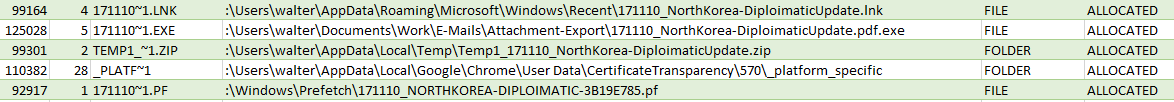
\includegraphics[width=15.8cm]{figures/mft.png}
	\captionof{figure}{MFT-Datei}
	\label{fig:mft}
\end{center}

\section{Prefetch-Files}
Mithilfe des Tools PECmd wurde das zur Malware gehörende Prefetch-File \path{/Windows/Prefetch/171110_NORTHKOREA-DIPLOIMATIC-3B19E785.pf} analysiert. Das Ergebnis ist in Abbildung \ref{fig:prefetch}
Es konnte nachgewiesen werden, dass die Malware zuletzt am 13.11.17 um 16:27 Uhr ausgeführt wurde. Dies lässt den Schluss zu, dass der Client des Mitarbeiters schon einen Tag vor dem Security Incident am 14.11.17 kompromittiert war.

\begin{center}
	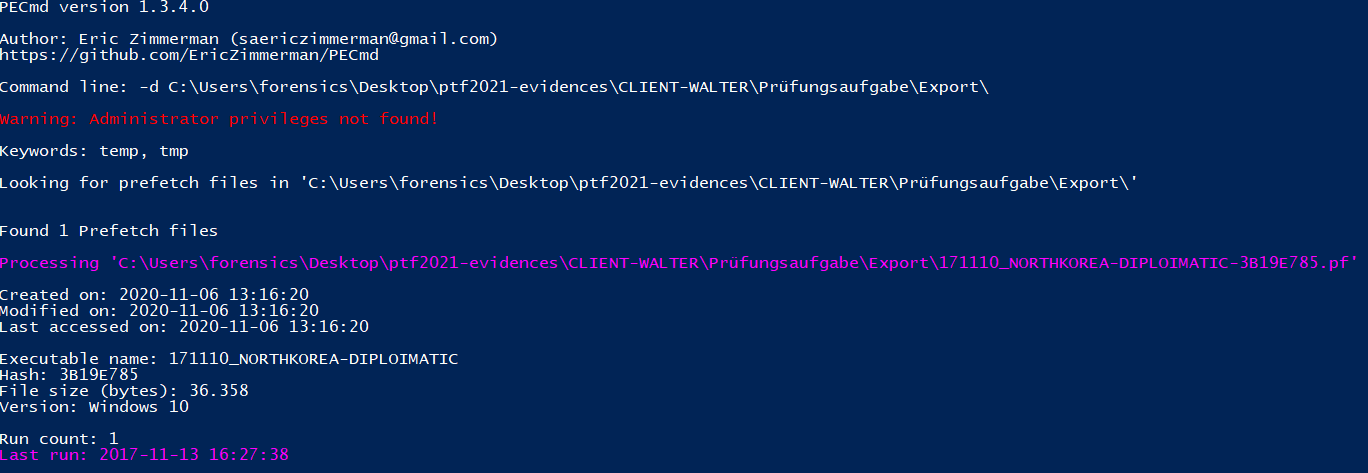
\includegraphics[width=15.8cm]{figures/prefetch.png}
	\captionof{figure}{Prefetch-Datei}
	\label{fig:prefetch}
\end{center}

\section{Registry-Analyse}
Es wurde eine Analyse der Registry Dateien NTUSER.dat, SYSTEM.dat, SAM.dat, SECURITY.dat und SOFTWARE.dat durchgeführt. Diese Dateien wurden aus dem Dateisystem des kompromittierten Rechners extrahiert und mit dem Programm RegRipper analysiert.
Die NTUSER Datei enthielt folgenden Eintrag unter dem Abschnitt UserAssist:
\\
\begin{center}
	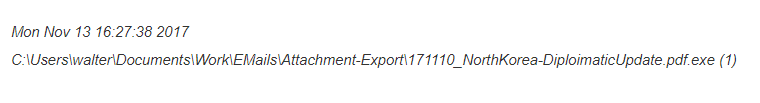
\includegraphics[width=15.8cm]{figures/prefetch_path.png}
	\captionof{figure}{Pfad zur verdächtigen Datei}
	\label{fig:prefetch_path}
\end{center}
\newpage
Diese Datei konnte aus dem Dateisystem des betroffenen Rechners extrahiert werden und wurde mit VirusTotal analysiert. In Abbildung \ref{fig:vtprefetch}  sind die Ergebnisse von VirusTotal zu sehen.

\begin{center}
	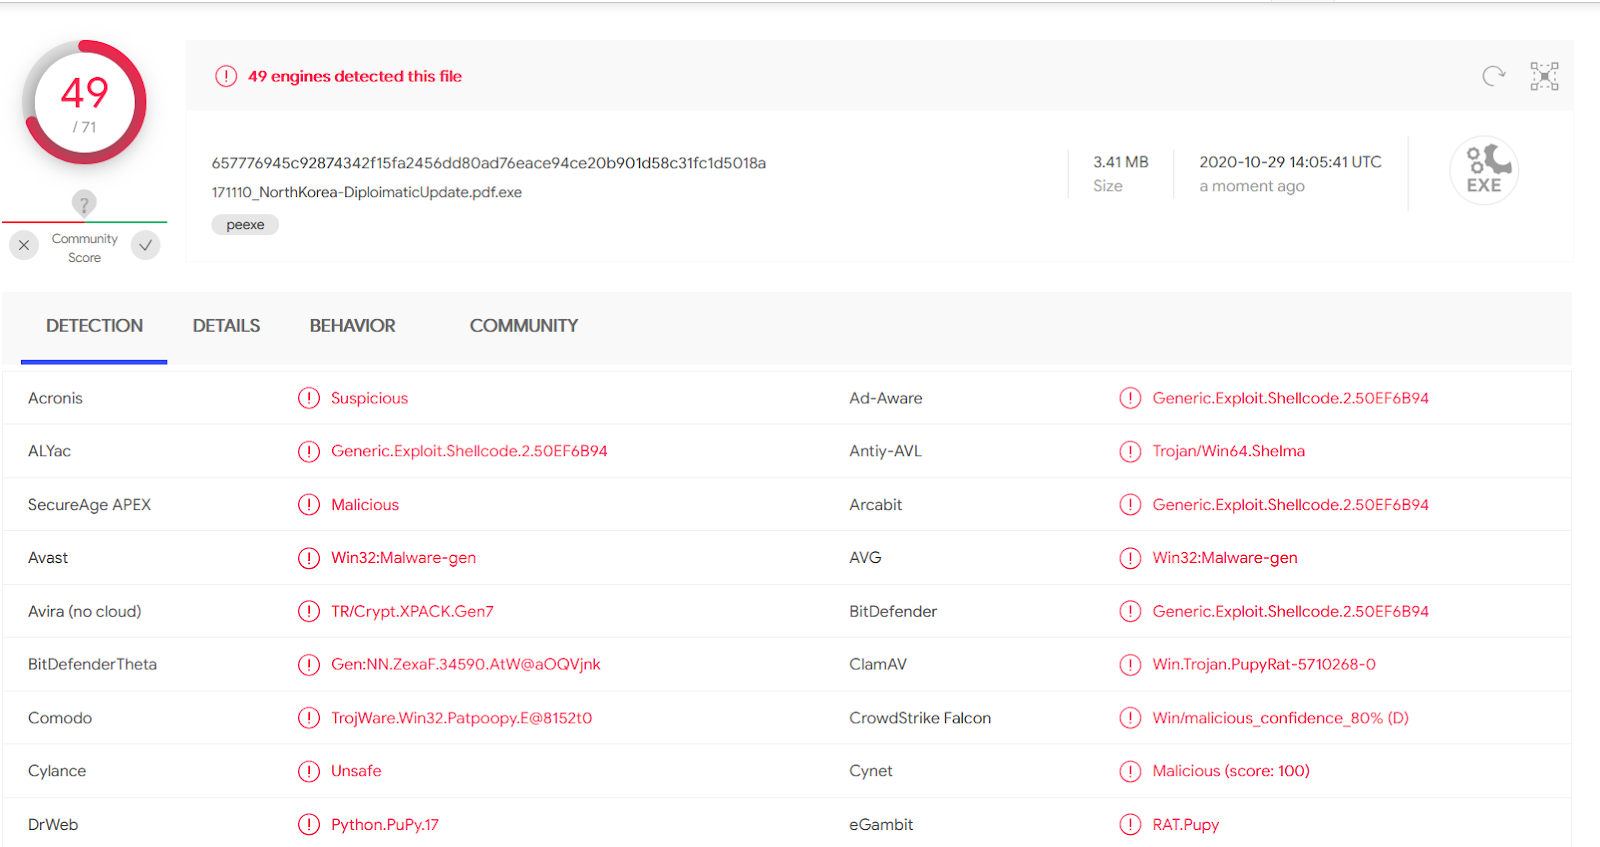
\includegraphics[width=15.8cm]{figures/virustotal_prefetch.png}
	\captionof{figure}{VirusTotal Scan der Malware 17110\_NorthKorea-DiploimaticUpdate\.pdf\.exe}
	\label{fig:vtprefetch}
\end{center}

Zusätzlich wurde in der \textit{NTUSER.dat} Datei der Key \textit{RecentDocs} analysiert. Es stellte sich dabei heraus, dass diese Datei zum letzten Mal am \textit{1. Januar 1970, 00:00 Uhr} geschrieben wurde.
Es ist zu vermuten, dass der Angreifer das Attribut \textit{LastWrite} bewusst auf den Beginn der Unixzeit gesetzt hat, was auf eine Manipulation zur Verschleierung von Spuren hindeuten könnte.
Ein Ausschnitt aus der RecentDocs-Analyse ist in Abbildung \ref{fig:RecentDocs} zu sehen.
Die SECURITY.dat und SAM.dat Dateien enthielten keine aufschlussreichen Einträge.

\begin{center}
	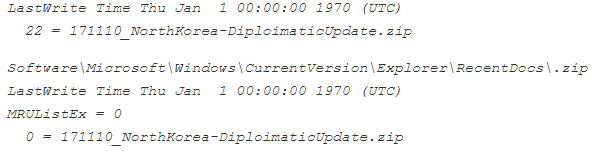
\includegraphics[width=15.8cm]{figures/prefetch_manipulation.png}
	\captionof{figure}{Ausschnitt aus der RecentDocs-Analyse}
	\label{fig:RecentDocs}
\end{center}

\newpage
Um den letzten Login im System festzustellen, wurde die Registry-Datei \textit{SOFTWARE.dat} analysiert.
Dabei stellte sich ebenfalls raus, dass der Eintrag Winlogon überschrieben wurde.
Auch hier ist davon auszugehen, dass der Angreifer diesen Eintrag überschrieben hat, um seine Spuren zu verwischen.
Der zuletzt eingeloggte User sowie der Zeitpunkt des Logins konnten somit nicht ermittelt werden. Dies ist in Abbildung \ref{fig:softwaredat} zu sehen.

\begin{center}
	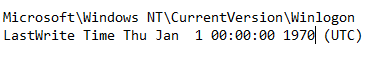
\includegraphics[width=15.8cm]{figures/softwaredat.png}
	\captionof{figure}{Ein Ausschnitt aus der Software.dat Analyse}
	\label{fig:softwaredat}
\end{center}

Die Ermittlungen ergaben, dass neben den bereits erwähnten Manipulationen, weitere Zugriffszeiten in allen Registry-Einträgen zurückgesetzt wurden.

\section{Wireshark Analyse}
Wireshark wurde am 13.11.17 um 16:24 Uhr herunterladen und eine Minute vor der eigentlichen Malware um 16:26 Uhr gestartet.
Dies geht aus der Analyse der Registry-Einträge hervor (siehe Abbildung \ref{fig:wireshark_paths}).

\begin{center}
	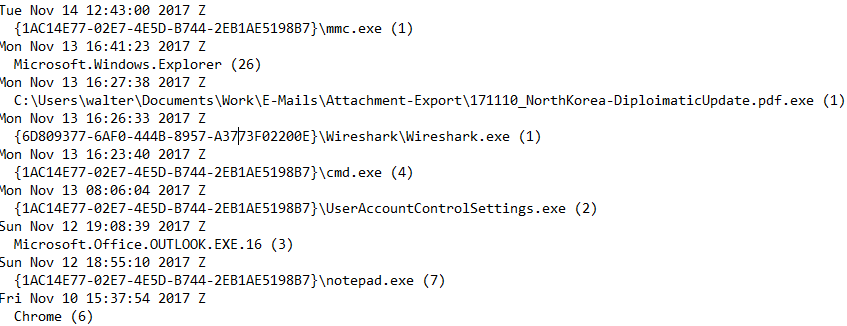
\includegraphics[width=15.8cm]{figures/wireshark_paths.png}
	\captionof{figure}{Ausschnitt der Registry-Einträge}
	\label{fig:wireshark_paths}
\end{center}

Es deutet darauf hin, dass der Mitarbeiter aufgrund eines ersten Verdachts das Sniffing-Tool selbst heruntergeladen hat, um den Netzwerkverkehr seines Rechners zu überwachen.
Die Browser-History zeigt, dass die Wireshark-Erweiterung \textit{Solarwinds Response Time Viewer} installiert wurde (siehe Abbildung \ref{fig:wireshark_history}).
Im Image des Users findet sicher unter \path{/root/Install} zwei Wireshark Dumps \path{dump_a.pcapng} und \path{dump_b.pcapng}.
Bei der Analyse der Wireshark Dumps fiel auf, dass die IP Adresse 192.168.8.131, welche eine gängige Adresse für Admin Interfaces ist, häufig aufgerufen wurde und dabei verschiedene Ports angesprochen wurden.
Dies deutet darauf hin, dass sich der Angreifer Zugang zur Admin-Konsole des Routers verschaffen wollte.
Es konnte kein Beweis gefunden werden, dass der Virus den Router kompromittieren konnte, es ist aber trotzdem dringend empfohlen den Router zu untersuchen.

\begin{center}
	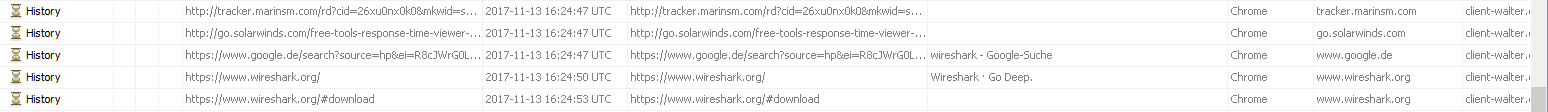
\includegraphics[width=15.8cm]{figures/wireshark_history.PNG}
	\captionof{figure}{Ausschnitt der Browser-History mit Autopsy}
	\label{fig:wireshark_history}
\end{center}

\section{Arbeitsspeicheranalyse}
Mithilfe von \textit{Volatility 2.6.1} konnten aus dem Arbeitsspeicher die aktiven und beendeten Prozesse ausgewertet werden.
Dabei fiel auf, dass der verdächtige Prozess \path{171110_NorthKo} am 13.11.17 um 16:27 Uhr gestartet wurde und bis zur Extraktion bzw. der forensischen Sicherung des Arbeitsspeichers nicht beendet wurde.
Dies bestätigt den Security Incident. Die Ausgabe von \textit{Volatility pslist} ist in Abbildung \ref{fig:processlist} zu sehen.
Eine Minute davor, um 16:26 Uhr, wurde Wireshark gestartet und am nächsten Tag, den 14.11.17, um 16:01 Uhr beendet.
Es ist zu vermuten, dass Wireshark vom Nutzer selbst ausgeführt wurde, da es vor dem Virus gestartet wurde.
Es ist zu empfehlen, den Mitarbeiter Lars Walter dazu zu befragen.

Es wurde in der Prozessanalyse mit Volatility der Prozess \path{171110_NorthKo} mit der Prozess-ID 6580 gefunden.
Wie in Abbildung \ref{fig:processlist} zu erkennen ist, hat dieser Prozess weitere Prozesse mit der Bezeichnung \textit{cmd.exe} gestartet.
Diese weisen alle die oben erwähnte PID 6580 der Malware als Parent-PID auf.
Obwohl diese Prozesse als verdächtig zu betrachten sind, konnte nicht eindeutig festgestellt werden, welche Funktion sie erfüllen.

\begin{center}
	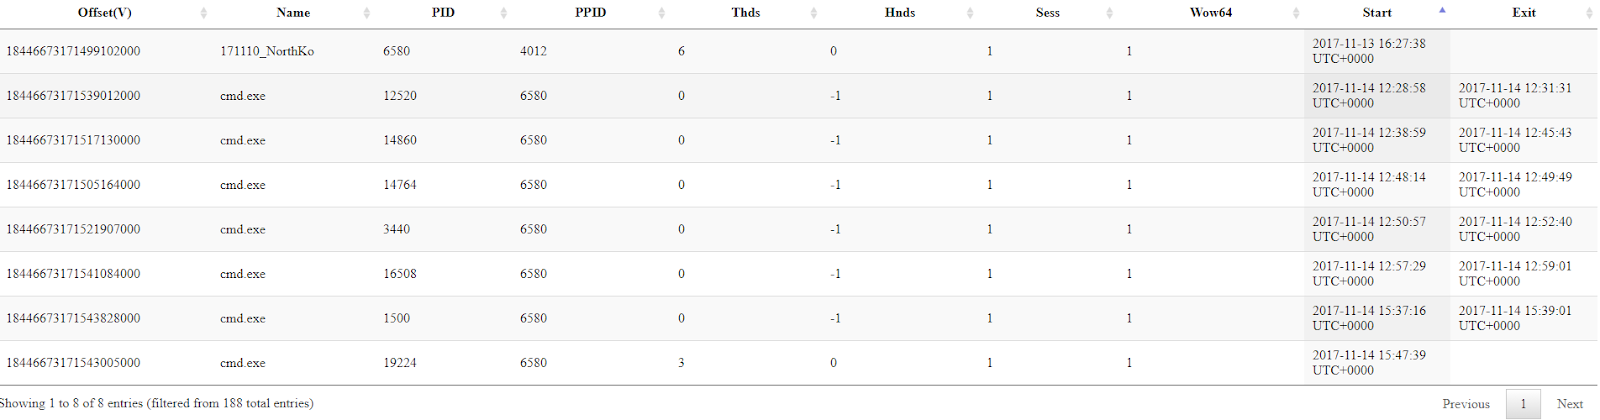
\includegraphics[width=15.8cm]{figures/processlist.png}
	\captionof{figure}{Prozessübersicht aus der Arbeitsspeicheranalyse}
	\label{fig:processlist}
\end{center}

\newpage
Wie in Abbildung \ref{fig:netscan} ersichtlich, konnte mit dem Plugin \textit{netscan} von Volatility herausgefunden werden, dass die Malware auf die IP-Adresse \path{210.122.17.27:80} zugreift.
Eine Whois-Abfrage der IP Adresse ergab, dass es sich um eine südkoreanische Adresse handelt.
Dies wird im Kapitel \ref{ch:Datendiebstahl} weiter untersucht.

\begin{center}
	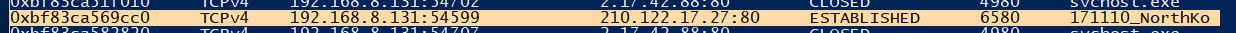
\includegraphics[width=15.8cm]{figures/netscan.png}
	\captionof{figure}{Ausschnitt aus dem Volatility-Plugin netscan}
	\label{fig:netscan}
\end{center}

Bei der Analyse mit dem Volatility Plugin \textit{handles} konnte herausgefunden werden, auf welche Registry-Schlüssel der besagte Prozess ein Handle besitzt (siehe Abbildung \ref{fig:handles}).
Nach dem Auslesen der jeweiligen Registry-Schlüssel konnten jedoch keine verdächtigen Einträge nachgewiesen werden.
Möglicherweise wurden auf diese Weise die Zeitstempel der Registry-Einträge zurückgesetzt.

\begin{center}
	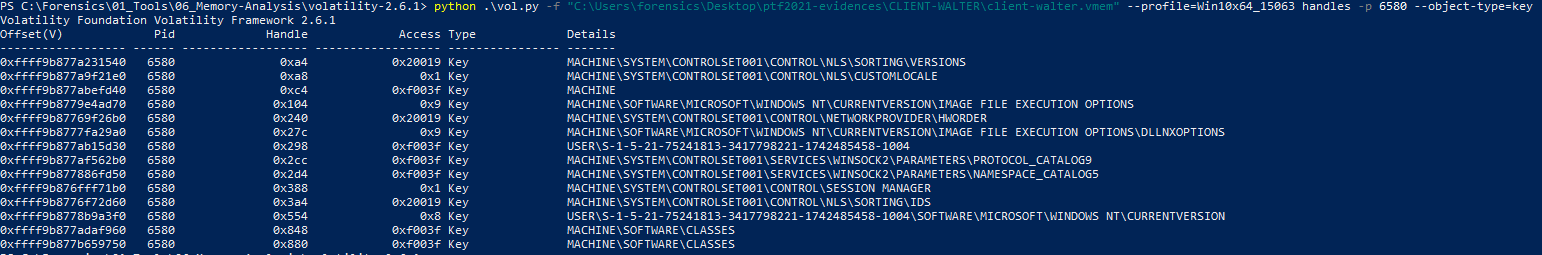
\includegraphics[width=15.8cm]{figures/volatility-handles.png}
	\captionof{figure}{Ausschnitt aus dem Volatility-Plugin handles}
	\label{fig:handles}
\end{center}

\chapter{Art des Angriffs}

Mithilfe von \textit{Autopsy} wurde der Browserverlauf sowie die E-Mail-Nachrichten des betroffenen Systems auf verdächtige Aktivitäten und Nachrichten analysiert. 
Im Posteingang (lokale Sicherung von Outlook) konnte dabei die Existenz einer Phishing-Mail nachgewiesen werden, welche am 13.11.17 um 16:19 Uhr empfangen wurde (siehe Abbildungen \ref{fig:outlook} und \ref{fig:email}).

\begin{center}
	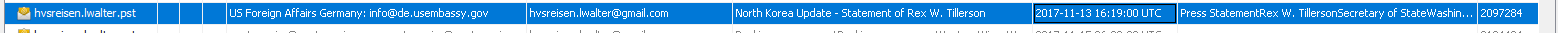
\includegraphics[width=15.8cm]{figures/outlook.png}
	\captionof{figure}{Ausschnitt des Posteingangs in Autopsy}
	\label{fig:outlook}
\end{center}

\begin{center}
	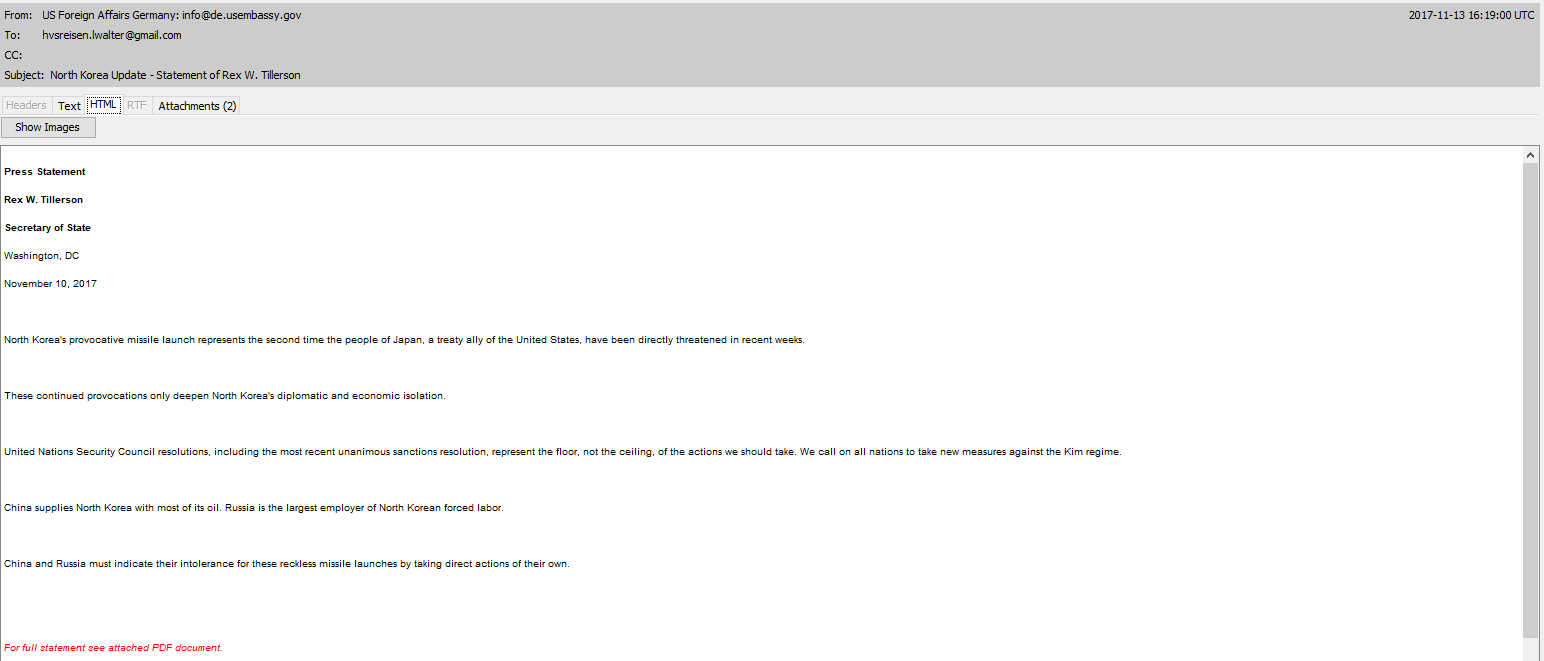
\includegraphics[width=15.8cm]{figures/email.png}
	\captionof{figure}{Ausschnitt der Phishing-Mail}
	\label{fig:email}
\end{center}

Im Mail-Anhang befand sich eine Zip-Datei, welche die auf dem System nachgewiesene Malware \path{171110_NorthKorea-DiploimaticUpdate.pdf.exe} enthielt (siehe Abbildung \ref{fig:email2}).
Mit großer Wahrscheinlichkeit ist anzunehmen, dass es sich bei der Phishing-Mail um einen gezielten Angriff auf hVs-reisen handelte.
Die Nachricht sollte dabei den Eindruck erwecken, sie stamme von einem hochrangigen Beamten des US-Außenministeriums und liefere wichtige Informationen über Änderungen der diplomatischen Beziehungen zu Nordkorea.
Vor dem Hintergrund des Geschäftsmodells von hVs-reisen (Reisen nach Nordkorea), ist anzunehmen, dass der betroffene Mitarbeiter sich dazu verleiten ließ, die E-Mail als seriös zu betrachten und den Anhang zu öffnen.

\begin{center}
	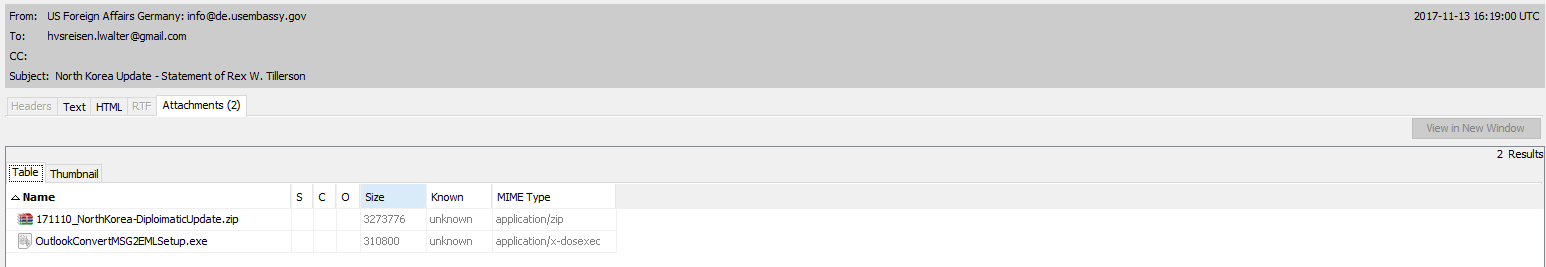
\includegraphics[width=15.8cm]{figures/email2.png}
	\captionof{figure}{Ausschnitt des Anhangs der Phishing-Mail}
	\label{fig:email2}
\end{center}

Ferner konnte nachgewiesen werden, dass am 12.11.2017 ab 18:55 Uhr mehrfach über den Webbrowser des Mitarbeiters auf dessen E-Mail-Postfach \path{hvsreisen.lwalter@gmail.com} zugegriffen wurde.
Dabei wurde um 19:47 Uhr der Zugriff für weniger sichere Apps auf den Google E-Mail Account des Mitarbeiters aktiviert (siehe Abbildung \ref{fig:lesssecure}).
Ob diese Änderung absichtlich erfolgte, kann nur durch weitere Befragung des Mitarbeiters ermittelt werden.
Sollte sich dabei herausstellen, dass die Einstellung nicht von ihm selbst durchgeführt wurde, liegt die Vermutung nahe, dass der Angreifer bereits vor der Phishing-Attacke Zugriff auf das E-Mail Konto des Mitarbeiters hatte, was die Bedrohungslage als Ganzes massiv erhöhen würde.
Für eine endgültige Bestätigung müsste dieser Annahme in einem separaten Projekt weiter nachgegangen werden.

Unabhängig von der Frage, wer die konkrete Änderung durchführte, wurde dadurch die Sicherheit des Systems gefährdet. Die Einstellung erlaubt nämlich Anwendungen, die nicht dem Sicherheitsstandard von Google entsprechen, den Zugriff auf das Postfach.

\begin{center}
	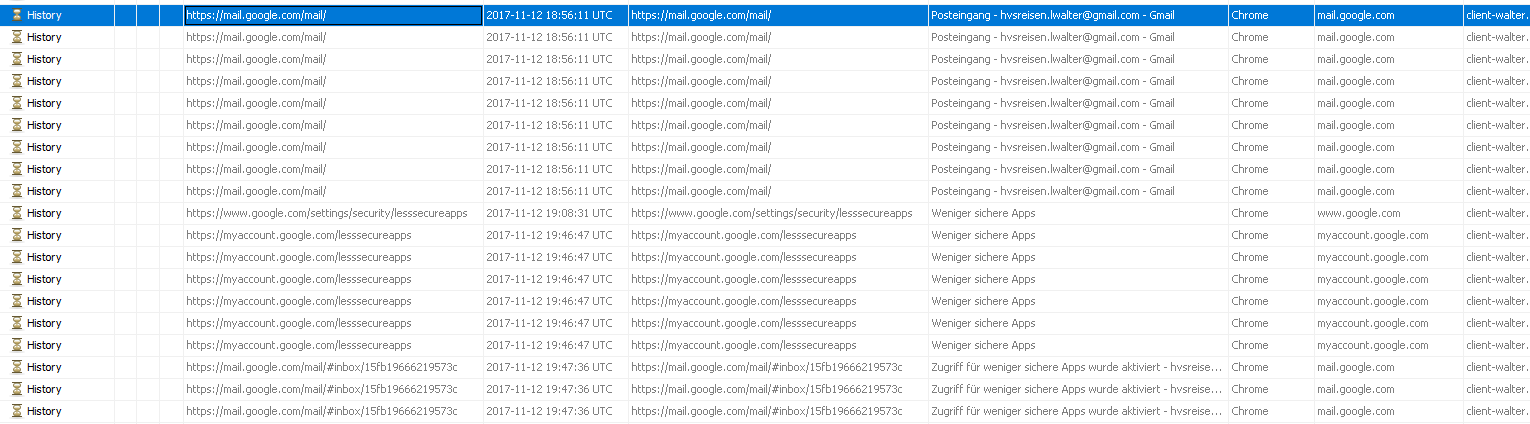
\includegraphics[width=15.8cm]{figures/lesssecure.png}
	\captionof{figure}{Ausschnitt des Browser-Verlaufs mit Aufruf der Einstellung \textit{less secure apps}}
	\label{fig:lesssecure}
\end{center}

\chapter{Weitere Aktivität des Angreifers}
Mithilfe der Timeline-Funktionalität des Forensik-Tools \textit{Autopsy} wurde die verdächtig wirkende Datei \textit{fklmjsvktiq.exe} gefunden (siehe Abbildung \ref{fig:malware-fklm}).
Diese Datei wurde am 13.11.17 um 16:53 Uhr im Dateisystem angelegt und ausgeführt.

\begin{center}
	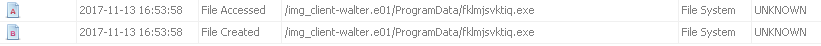
\includegraphics[width=15.8cm]{figures/malware-fklm.png}
	\captionof{figure}{Nachweis der Existenz von fklmjsvktiq.exe}
	\label{fig:malware-fklm}
\end{center}

Zur weiteren Analyse wurde die Datei auf \path{www.virustotal.com} hochgeladen.
Das Ergebnis des Scans ist in Abbildung \ref{fig:virustotaol-fkl} zu sehen.
Dabei stellte sich heraus, dass die Datei als Schadsoftware eingestuft wird. Anhand VirusTotal konnte außerdem das grobe Verhalten der Schadsoftware abgelesen werden.
\begin{center}
	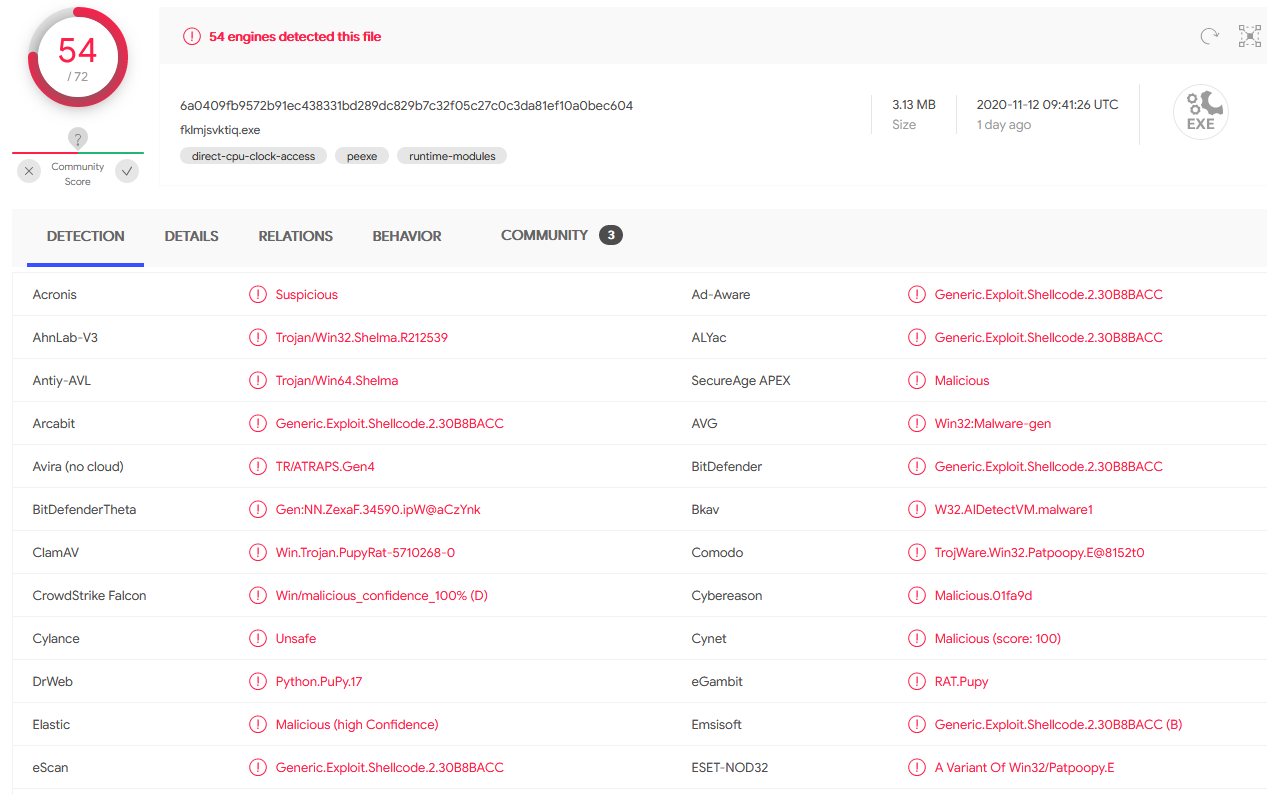
\includegraphics[width=15.8cm]{figures/virustotaol-fklm.PNG}
	\captionof{figure}{VirusTotal Auswertung zu fklmjsvktiq.exe}
	\label{fig:virustotaol-fkl}
\end{center}

\newpage
Es stellte sich dabei heraus, dass die Malware in der Lage ist, wichtige .dll Libraries wie kernel32.dll (Verwaltung von Speicher und  Ein-/Ausgabefunktionen) und user32.dll zu importieren, welche möglicherweise zu weitreichenden Eingriffen ins System genutzt wurden.
Des Weiteren werden verschiedene IP-Adressen aufgerufen wie in Abbildung \ref{fig:virustotal-fklm03} zu sehen ist, wobei die Adresse 210.122.17.27 auf einen koreanischen Server verweist und in vorliegenden Kontext daher besonders verdächtig erscheint.

\begin{center}
	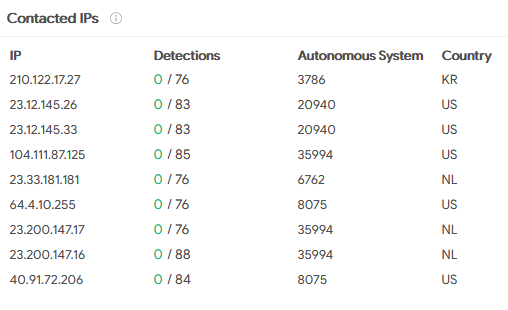
\includegraphics[width=15.8cm]{figures/virustotal-fklm03.PNG}
	\captionof{figure}{VirusTotal Analyse der aufgerufenen IP Adressen der fklmjsvktiq.exe}
	\label{fig:virustotal-fklm03}
\end{center}

Laut VirusTotal ist die Schadsoftware außerdem in der Lage, eine ausführbare Datei mit dem Namen oewjeya.exe zu erstellen (siehe Abbildung \ref{fig:oewja}).
Diese konnte allerdings nicht im System des Mitarbeiters nachgewiesen werden.

\begin{center}
	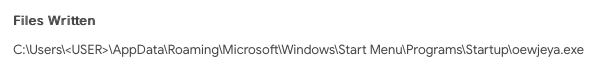
\includegraphics[width=15.8cm]{figures/oewja.png}
	\captionof{figure}{Ausschnitt aus VirusTotal für fklmjsvktiq.exe}
	\label{fig:oewja}
\end{center}

\chapter{Möglicher Datendiebstahl}
\label{ch:Datendiebstahl}
Die auf VirusTotal aufgeführten IP Adressen des Viruses wie in Abbildung \ref{fig:wiresharkanalysis} zu sehen, wurden in den Wireshark Dumps analysiert. Dabei wurde eine der Verbindungen auf die IP Addresse 210.122.17.27:80 gefunden. Es fiel auf, dass sehr viele Calls auf diese IP Adresse durchgeführt wurden. Dabei wurden auch Daten übertragen, da die Calls teilweise eine sehr hohe Größe hatten.

\begin{center}
	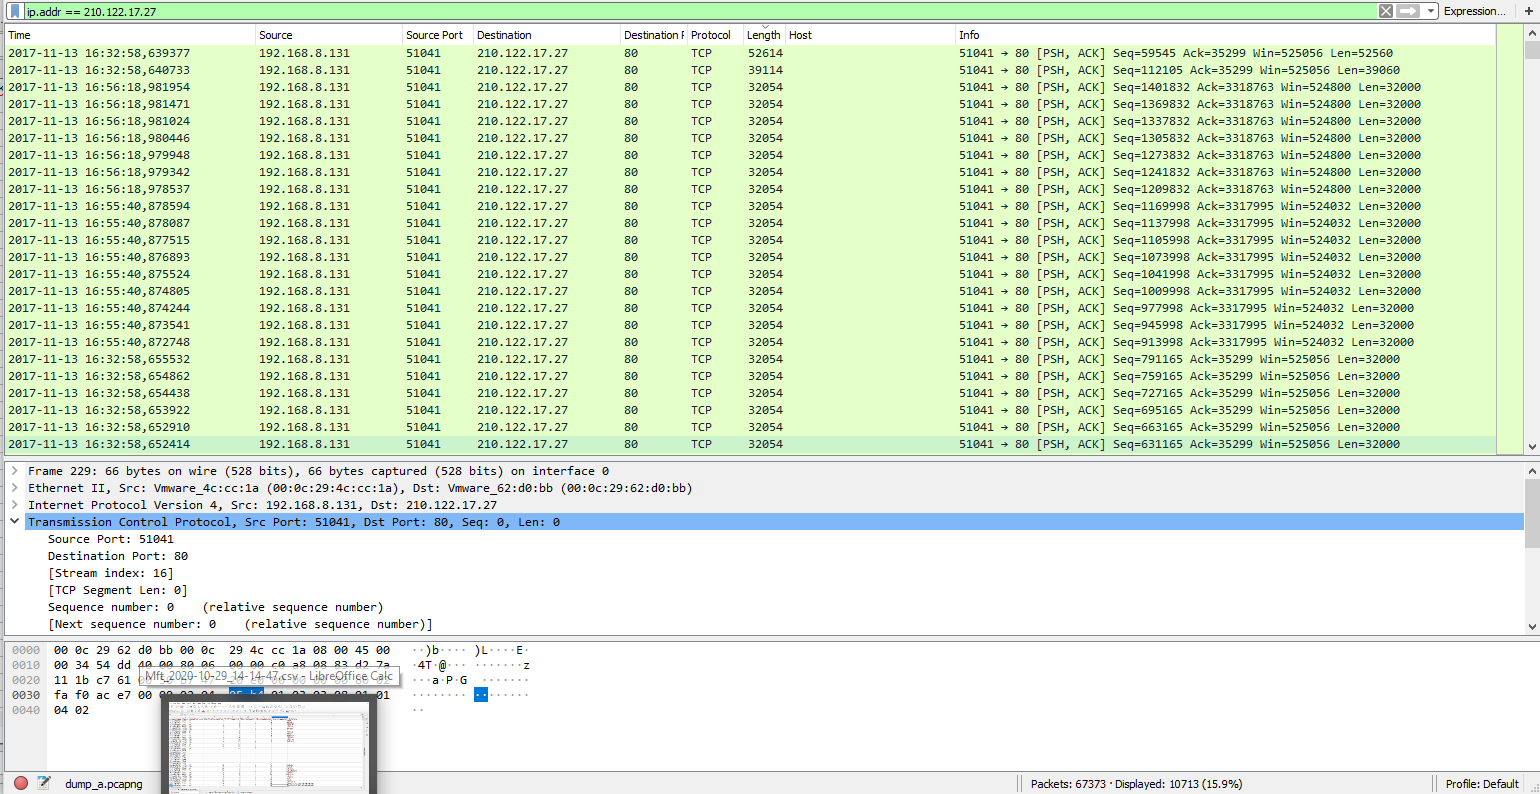
\includegraphics[width=15.8cm]{figures/wiresharkanalysis.png}
	\captionof{figure}{Wireshark Analyse der Calls auf 210.122.17.27:80}
	\label{fig:wiresharkanalysis}
\end{center}

In Abbildung \ref{fig:wiresharkanalysis} ist zu sehen, dass es insgesamt über 67000 Pakete mit Ziel oder Absenderadresse dieser IP Adresse hat und dass das größte Paket eine Länge von über 52000 Bytes hat. Dies deutet darauf hin, dass Daten hochgeladen wurden.

Per \textit{whois}-Abfrage konnte ermittelt werden, dass sie einem asiatischen Provider zuzuordnen ist, allerdings sind durch das hohe Alter, keine genaueren Angaben möglich. Es könnte mittlerweile neu vergeben worden sein oder dieser Server war auch betroffen und wurde nur als Mittelsmann genutzt.

\chapter{Empfohlene nächste Schritte für hVs-Reisen}

Dem betroffenen Mitarbeiter Lars Walter wird empfohlen, die Passwörter für sämtliche Accounts und Dienste zu ändern, bei denen er sich seit der Ausführung der Malware am 13.11.17 um 16:27 Uhr vom betroffenen Rechner aus eingeloggt hat.
Dringend geändert werden sollte das Passwort für den Google E-Mail Account, da nachgewiesen werden konnte, dass sich der Mitarbeiter nach dem Malware-Befall noch mehrfach bei diesem Dienst angemeldet hatte (siehe Abbildungen \ref{fig:history1} und \ref{fig:history2})

\begin{center}
	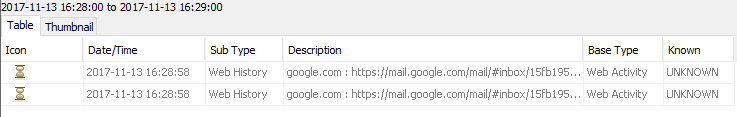
\includegraphics[width=15.8cm]{figures/history1.PNG}
	\captionof{figure}{Browserhistory des Nutzers}
	\label{fig:history1}
\end{center}

\begin{center}
	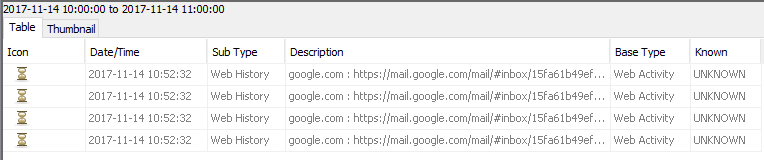
\includegraphics[width=15.8cm]{figures/history2.PNG}
	\captionof{figure}{Browserhistory des Nutzers}
	\label{fig:history2}
\end{center}

Der kompromittierte Rechner sollte vollständig neu aufgesetzt werden, da nicht auszuschließen ist, dass neben der gefundenen Malware noch weitere Schadsoftware installiert wurde.
Weiterhin sollte auch der Netzwerk-Router untersucht werden, um festzustellen, ob es dem Angreifer gelang, auf diesen Zugriff zu erlangen.
Auch das Passwort des Netzwerk-Routers sollte von der IT-Administration geändert werden.
Es empfiehlt sich, alle Passwörter der Mitarbeiter von hVs-Reisen zu ändern, da wir einen Zugriff auf weitere Accounts derzeit nicht ausschließen können.
Zudem sollten alle E-Mail Accounts der Mitarbeiter auf Aktivierung der \textit{Less secure apps} untersucht werden.

Zuletzt sollten alle Mitarbeiter für die IT-Sicherheit sensibilisiert werden, damit ein solcher Angriff auf hVs-Reisen in Zukunft vermieden werden kann.
Es sollte vor allem darauf hingewiesen werden, dass nicht direkt auf die Links der erhalten E-Mails geklickt wird.
Die Mitarbeiter sollen sich erst vergewissern, dass die E-Mail vertraulich ist.